\chapter{Research Methodology} \label{chp:method}

The methodology used to develop the grey box model will be discussed in this chapter. The grey box modelling approach in this thesis falls under the category of sequential GBM. Hence, the development process is divided into two stage. The first stage of the modelling focus on machine learning modelling i.e. BBM using tree-based model using python with help of \scikit/ \bcitep{FabianPedregosa.2011}. This includes the process of data acquisition, data preprocessing, hyperparameter optimisation and model evaluation. The training of the models utilises a fusion of T-AIS data and weather data, then, relevant features are selected to predict the SOG. These processes are visually presented in \Cref{fig:flowchart_BBM}.\\

\begin{figure}[h]
    \centering
        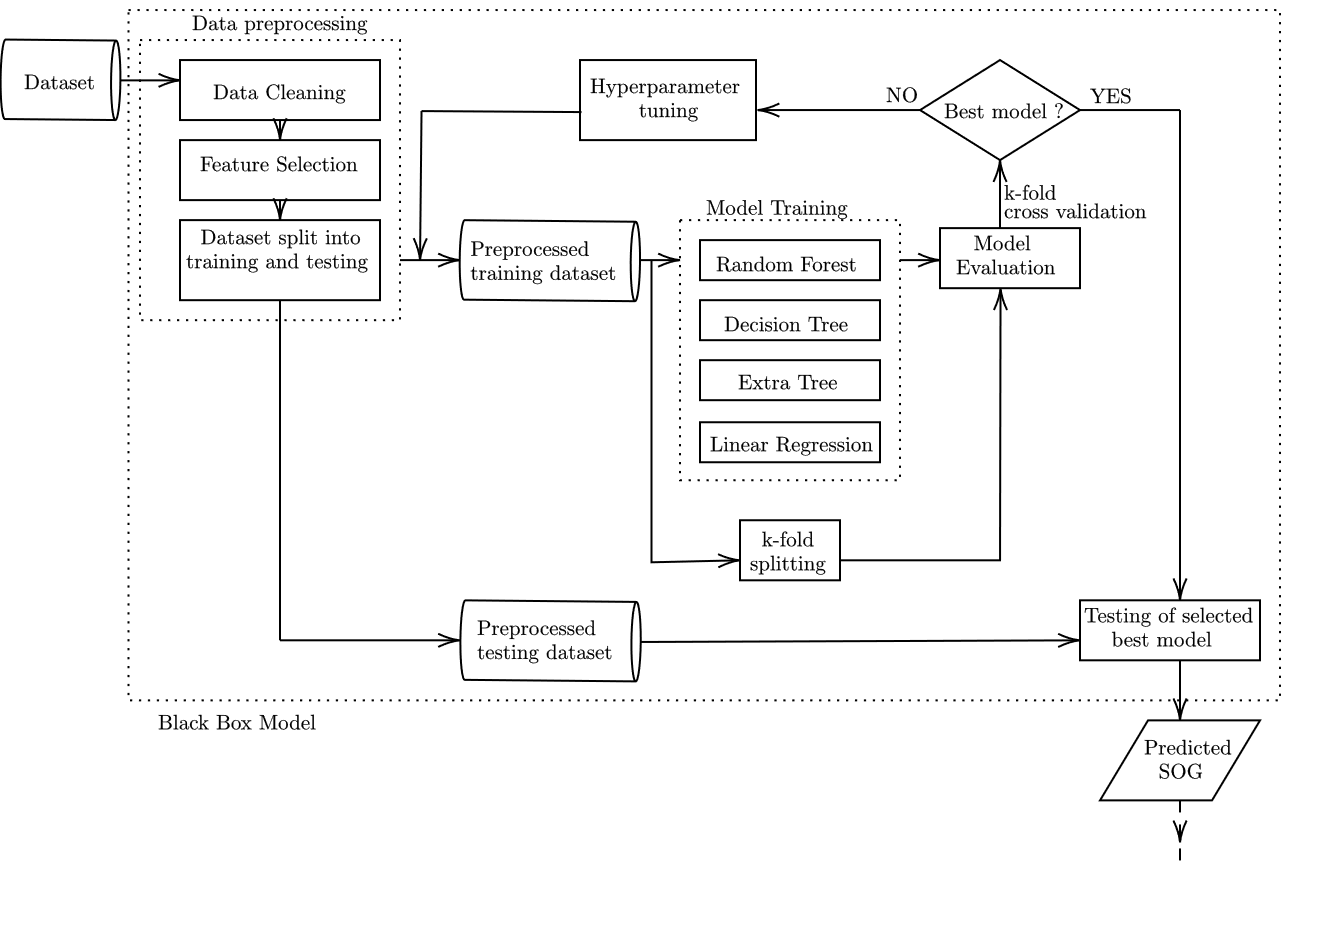
\includegraphics[width=\textwidth]{02_figures/flowmethod_BBM_alt.png}
        \caption{Scheme of proposed BBM methodology}
        \label{fig:flowchart_BBM}
\end{figure}

The second stage of the modelling focus on WBM aspect of the GBM. The predicted SOG will be fed into the WBM to predict the required brake power required to propulse the ship. The SOG will need to be first converted into STW for the resistance calculations and consequently power calculations. The framework presented in \Cref{fig:flowchart_WBM} refers is a graphical summary of \Cref{sec:power_calc}. 

\begin{figure}[h]
    \centering
        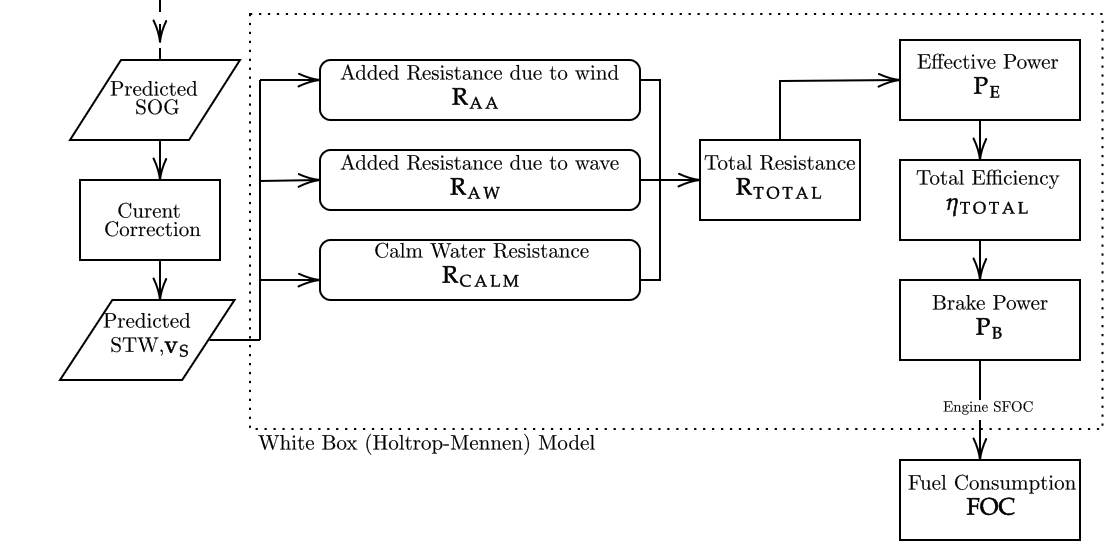
\includegraphics[width=\textwidth]{02_figures/flowmethod_WBM.png}
        \caption{Scheme of proposed WBM methodology adopted from \bcitet{XiaoLang.2020}}
        \label{fig:flowchart_WBM}
\end{figure}

The development process of GBM is summarised in \Cref{fig:flowchart_GBM}. Detailed discussion regarding the development of BBM and WBM model will be discussed in the following sections of this chapter.

\begin{figure}[h]
    \centering
        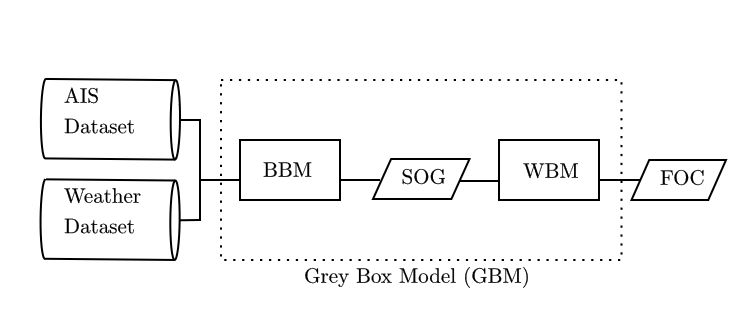
\includegraphics[width=.85\textwidth]{02_figures/flowmethod_GBM_alt.png}
        \caption{Scheme of proposed GBM methodology}
        \label{fig:flowchart_GBM}
\end{figure}


\section{Data Acquisition}\label{sec:data_acquisition}

The data is collected from a ferry serving between ports of K{\o}ge, R{\o}nne, Ystad and Sassnitz, as shown in \Cref{fig:Hammershus_journey_map} \bcitep{HammershusJourney}. The trip between K{\o}ge, R{\o}nne takes about 5 h 30 minutes and it sails between R{\o}nne and Sassnitz for 3 h and 20 minutes. The journey is tracked by T-AIS system of Danish Maritime Authority (DMA). The weather data along her sailing path are acquired from ECMWF\footnote{European Centre for Medium-Range Weather Forecast} with temporal resolution of 1 hour at granularity of 0.25° (longitude) x 0.25° (latitude), data from ECMWF provides information for wind, waves and seawater temperature. The information for current is obtained from CMEMS\footnote{Copernicus Marine Environment Monitoring Service} with temporal resolution of 3 hours at granularity of  0.25° (longitude) x 0.25° (latitude).\\ 

\begin{figure}[ht]
  \begin{minipage}{0.55\linewidth} % Adjust the width as needed
    \footnotesize
    \centering
    \begin{tabular}{l r}
        \hline
        IMO & 9812107 \\
        Type \& Service & Passenger ferry \\
        $L_{OA}$ & 158.00 m\\
        $L_{WL}$ & 144.80 m\\
        $B$ (moulded) & 24.5 m\\
        $T_{DESIGN}$ & 5.70 m\\
        $T_{MAX}$ & 5.85 m \\ 
        Gross Tonnage (GT) & 18,009 \\
        Deadweight (dwt) & 4,830 t \\
        Main Engines & Wärtsillä 8V31 2 x 4,880 kW \\
        SFOC & 169.4 g/kWh \\
        Service Speed & 17.7 knots \\
        Bow Thrusters & 2 x 1500 kW \\
        \hline
    \end{tabular}
    \caption{Particular of M/S Hammershus}
    \label{tbl:Hammershus_Data}
  \end{minipage}
  \hspace{0.01\linewidth}
%   \hfill
  \begin{minipage}{0.43\linewidth} % Adjust the width as needed
    \centering
    % \vspace*{0.1cm}
    \includegraphics[width=\linewidth]{02_figures/Bornholmerfærgen_route_map.png} % Replace example-image.jpg with your picture file name
    \caption{Journey of the ferry}
    \label{fig:Hammershus_journey_map}
  \end{minipage}
\end{figure}


\begin{figure}[h]
    \centering
        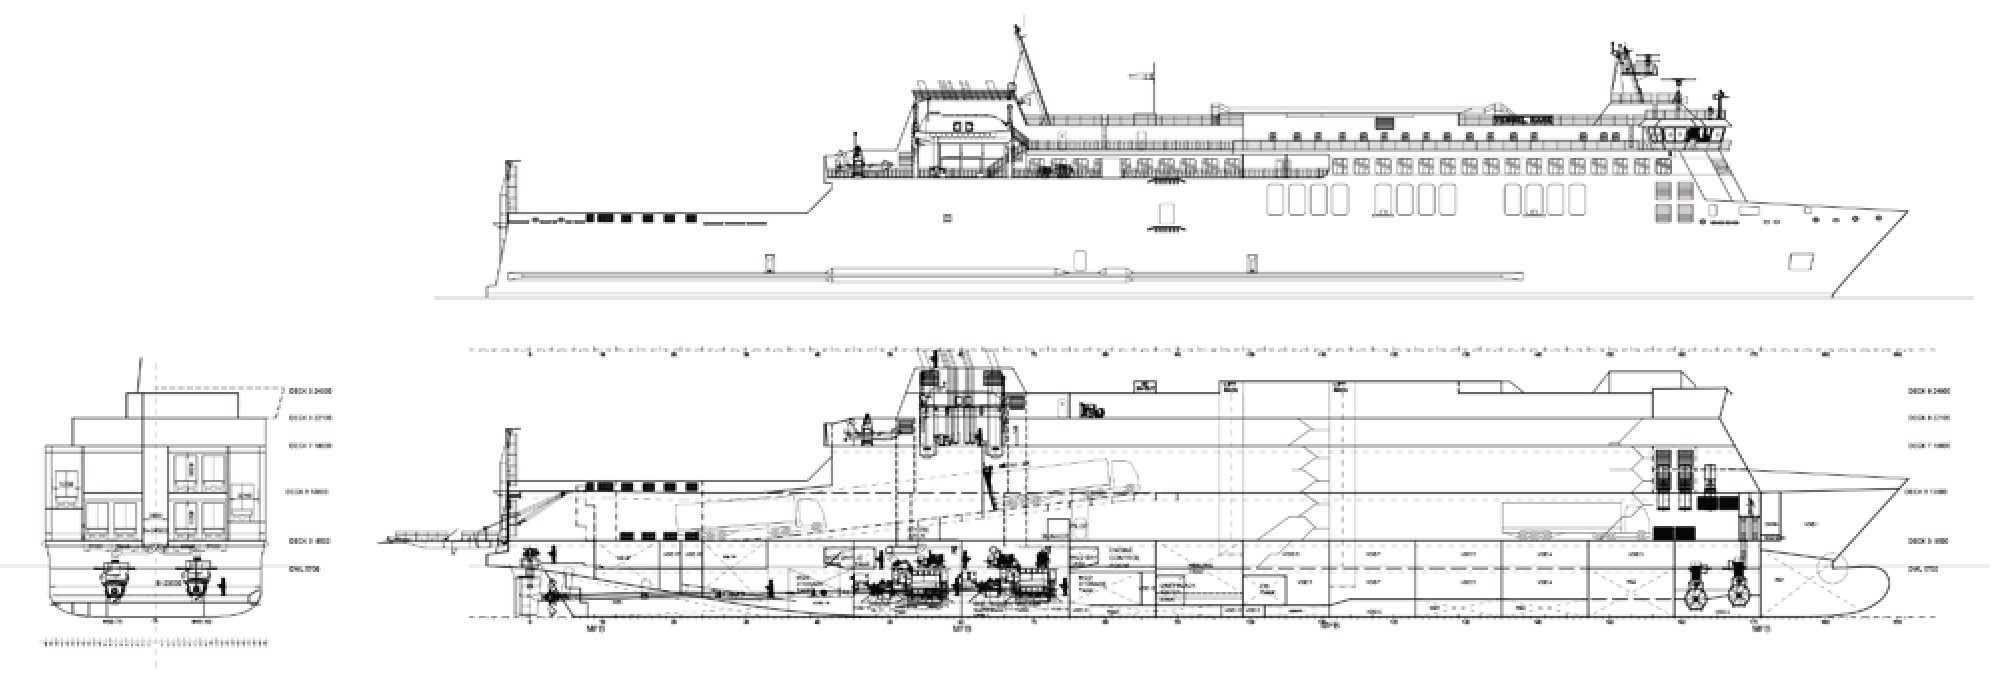
\includegraphics[width=\textwidth]{02_figures/Hammershus_Pict.jpg}
        \caption{Schematics of M/S Hammershus}
        \label{fig:Hammershus_Pict}
\end{figure}

The resulting fused dataset has a temporal resolution of 1 hour. Due to the difference in temporal resolution of the data from CMEMS and ECMWF, the weather information is synchronised so that the wind, waves, seawater temperature and sea current belongs to the same weather grid with same temporal resolutions. The features \textbf{wind direction},\textbf{swell direction}, and \textbf{wind wave direction} are oriented to true north. However, to reflect the actual direction of weather effects that are acting on the ship, these features are converted to true direction; where true direction is defined as the direction of weather effect with respect to the bow of the ship. The value ranges between 0° and 180°. Subsequently, through vector decomposition, the northward and eastward wind velocity is converted to absolute wind speed and wind direction \emph{with respect to True North},$\varphi$:

\begin{equation}\label{eqn:vwindabs}
    V_{\text{wind}} = \sqrt{(V_{\text{wind}}^N)^2 + (V_{\text{wind}}^E)^2} 
\end{equation}
\begin{equation}\label{eqn:winddir}
    \varphi = 
    \begin{cases}
        360 - \arctan(\frac{V_{\text{wind}}^E}{V_{\text{wind}}^N}) \quad \text{\textbf{if}} \quad V_{\text{wind}}^E > 0 \quad \wedge \quad V_{\text{wind}}^N < 0 \\ 
        180 - \arctan(\frac{V_{\text{wind}}^E}{V_{\text{wind}}^N}) \quad \text{\textbf{if}} \quad V_{\text{wind}}^E < 0 \quad \wedge \quad V_{\text{wind}}^N > 0 \\ 
        270 - \arctan(\frac{V_{\text{wind}}^E}{V_{\text{wind}}^N}) \quad \text{\textbf{if}} \quad V_{\text{wind}}^E > 0 \quad \wedge \quad V_{\text{wind}}^N > 0 \\
        \arctan(\frac{V_{\text{wind}}^E}{V_{\text{wind}}^N}) \qquad \text{\textbf{otherwise}} 
    \end{cases}   
\end{equation}

Similarly, information of Northward and Eastward current Velocity is converted to absolute current speed and current direction \emph{with respect to True North} $\gamma$.\\ 

\begin{equation}\label{eqn:vcurrabs}
    V_{\text{current}} = \sqrt{(V_{\text{current}}^N)^2 + (V_{\text{current}}^E)^2} 
\end{equation}
\begin{equation}\label{eqn:currdir}
    \gamma = 
    \begin{cases}
        360 - \arctan(\frac{V_{\text{current}}^E}{V_{\text{current}}^N}) \quad \text{\textbf{if}} \quad V_{\text{current}}^E < 0 \quad \wedge \quad V_{\text{current}}^N > 0 \\ 
        180 - \arctan(\frac{V_{\text{current}}^E}{V_{\text{current}}^N}) \quad \text{\textbf{if}} \quad V_{\text{current}}^E > 0 \quad \wedge \quad V_{\text{current}}^N < 0 \\ 
        270 - \arctan(\frac{V_{\text{current}}^E}{V_{\text{current}}^N}) \quad \text{\textbf{if}} \quad V_{\text{current}}^E < 0 \quad \wedge \quad V_{\text{current}}^N < 0 \\
        \arctan(\frac{V_{\text{current}}^E}{V_{\text{current}}^N}) \qquad \text{\textbf{otherwise}} 
    \end{cases}   
\end{equation}

The initial dataset provides information to the true directions, which indicate the encounter direction of weather conditions with respect to the ship bow. Static information from the AIS data which only indicated the ship's identity and navigational status are discarded in the dataset. The initial structure have 27 features, 9 AIS features and 18 weather features. The structure of the initial dataset i.e. before data preprocessing and feature selection, is summarised in \Cref{tbl:dataset_init_struct} \\

\begin{table}[ht]
    \footnotesize
    \centering
    % \resizebox {\textwidth}{!}
    {\begin{tabular}{ p{0.4\textwidth} c }
    \hline
    \textbf{Feature} & \textbf{Feature Name}  \\
    \hline
    \multicolumn{2}{l}{\textbf{AIS data}}\\
    \hline
    Position Time Stamp [DD\slash MM\slash YYYY HH:MM:SS] & {\tt Time} \\
    Latitude [°] & {\tt LAT}   \\
    Longitude [°] & {\tt LON}  \\
    Width [m] & {\tt width}  \\
    Length [m] & {\tt length}\\
    SOG [Knots] & {\tt sog} \\
    COG [m/s] & {\tt cog}  \\
    Heading [°] & {\tt heading}  \\
    Draught [m] & {\tt draught} \\
    \hline
    \multicolumn{2}{l}{\textbf{Weather Data (0.5° Granularity)}}\\
    \hline
    Wind Speed [m/s] & {\tt windspeed} \\
    True North Wind Direction, $\varphi$ [°] & {\tt truenorthcurrentdir} \\
    Air Temperature Above Oceans [K] & {\tt oceantemperature} \\
    % Air Density Above Oceans [$\text{kg/m}^3$]& - \\
    Maximum Wave Height [m] & {\tt waveheight} \\
    % Swell Direction [°] & - \\
    % Wind Wave Direction & - \\
    Swell Period [s] & {\tt swellperiod} \\
    Wind Wave Period [s] & {\tt windwaveperiod}\\
    % Wave Direction [°] & - \\
    Wave Period [s] & {\tt waveperiod}\\
    Sea Surface Temperature [K] & {\tt surftemp}\\
    Combined Wind Wave Swell Height [m] &  {\tt windwaveswellheight} \\
    Swell Height [m] & {\tt swellheight}\\
    Wind Wave Height [m] & {\tt windwaveheight}  \\
    % Surface Pressure & - \\
    Current Speed [m/s] & {\tt curspeed} \\
    True North Current Direction $\gamma$ [°] & {\tt truenorthcurrentdir}\\
    True Wind Direction [°] & {\tt truewinddir}  \\
    True Current Direction [°] & {\tt truecurrentdir} \\
    True Swell Direction [°] & {\tt trueswelldir} \\
    True Wind Wave Direction [°] & {\tt truewindwavedir} \\
    True Wave Direction [°] & {\tt truewavedir} \\
    \end{tabular}}
\caption{Structure of fused dataset}\label{tbl:dataset_init_struct}
\end{table}

\section{Data Preprocessing}\label{sec:data_prep}

This section presents the steps taken during data preprocessing. The dataset will be subjected to data cleaning which include identification of anomalies and missing values. SOG threshold is applied to ensure that the model represent operating condition at steady state. Domain knowledge based, feature selection is performed to ensure the model does not violate vessel domain knowledge. The datasets then will be split to training, validation and test dataset. 

\subsection{Data Cleaning}\label{sec:data_cleaning}

The plot of the journey indicates that the journey between R{\o}nne and Sassnitz is not represented completely. This might be caused due to the limitation of T-AIS system which is caused by the due to poor coverage in the area between Sassnitz and R{\o}nne. This is shown by the plot shown in \Cref{fig:aiscoverage}. Therefore, the data plot for the journey between Sassnitz and R{\o}nne will be excluded. Basic threshold of decimal degrees of 55.04° N for latitude is applied, this threshold will exclude the journey between Sassnitz and R{\o}nne.\\

\begin{figure}
    \centering
        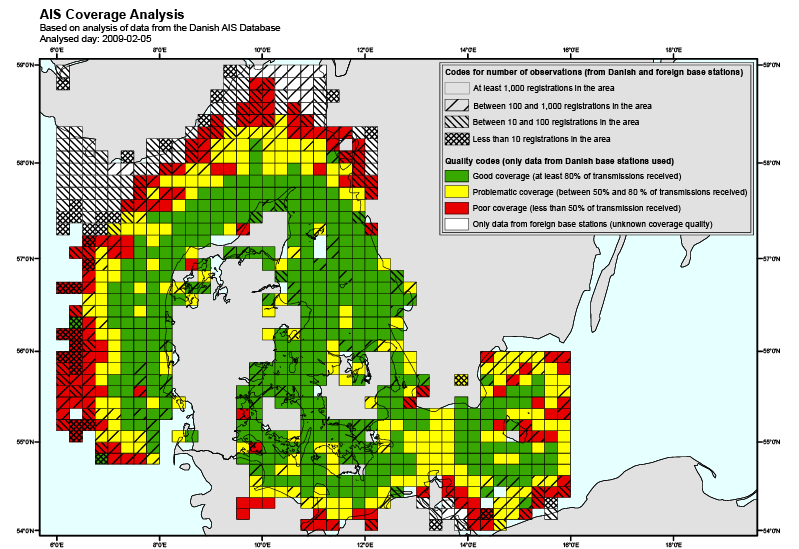
\includegraphics[width=0.8\textwidth]{02_figures/AIS_Coverage.png}
        \caption{Shore based AIS Coverage based on data from AIS database \cite{webaisdk.2023}}
        \label{fig:aiscoverage}
\end{figure}

In its initial state, the dataset contains 7453 data points which described the journey of the ship in one year. The initial data points represented all navigational status of the ship, which include ``mooring'', ``anchoring'' and ``underway using engine''. This is clearly observed in the histogram for the SOG \Cref{fig:anomalies_sog_curspeed}.\\ 

To ensure that the dataset represents the actual operating condition of ship in steady state, a threshold for SOG must be applied. SOG can vary due to changing sea state, but it can also be reduced by the ship's operator around the port when it departs from port of origin or arriving at port of arrival. Therefore, any data points with SOG less than 5 knots will be discarded which is considered as manoeuvring \bcitep{Abebe.2020,Yan.2020}. Post filtering, the amount of data points decrease significantly from 7453 data points to 3828 data points. This indicated that about half of the total data points represented the ship's stationary behaviour.\\

% \begin{figure}
%     \centering
%         \includegraphics[width=0.8\textwidth]{02_figures/SassnitznoFilter.png}
%         \caption{Journey of the ship in a year}
%         \label{fig:YearJourney}
% \end{figure}
\begin{figure}[h]
    \centering
        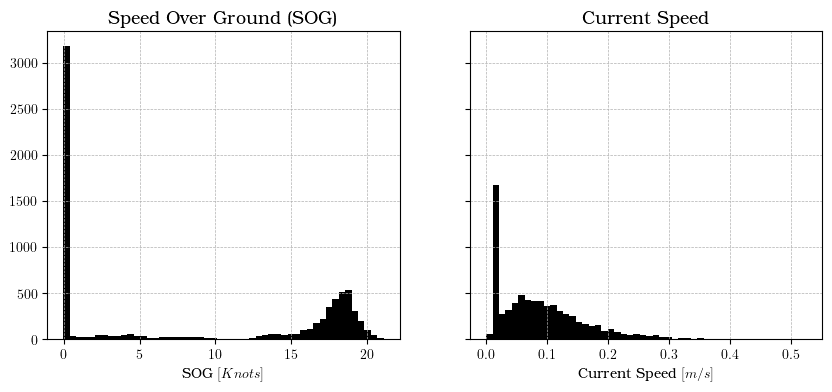
\includegraphics[width=0.9\textwidth]{02_figures/sog_curspeed_anomalies.png}
        \caption{Histogram plot of pre-filtered SOG and current speed}
        \label{fig:anomalies_sog_curspeed}
\end{figure}

From preliminary analysis, possible source of error is identified for data points representing current speed. In range of current speed between 0.01 and 0.03 $m/s$, noticeable peak in data points is observed as shown in \Cref{fig:anomalies_sog_curspeed}. This peak attributed to missing information on northward and eastward current speed in some data points from the provided dataset. This resulted in single random error value for current speed which resulted in the peak observed in the histogram.\\ 

\begin{figure}[h]
    \centering
        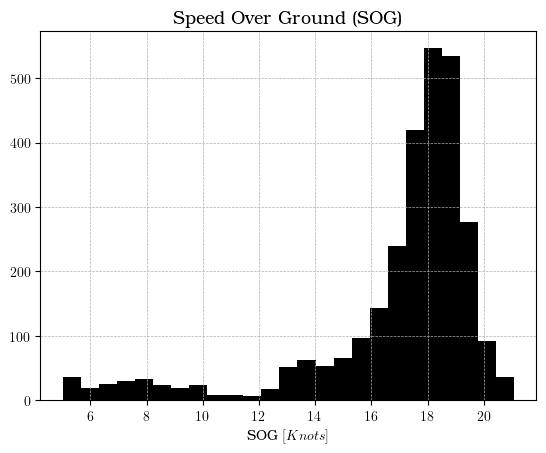
\includegraphics[width=0.6\textwidth]{02_figures/hist_init_sog_postfilter.png}
        \caption{Histogram plot of SOG after threshold}
        \label{fig:SOG_greater_five}
\end{figure}

To address the missing values, the missing values for eastward current and northward current are imputed using {\tt KNNImputer} feature from \scikit/. This is necessary as modelling package by \scikit/ cannot handle missing values. During imputing, each sample's missing values are imputed using the mean of nearest neighbour found in training dataset \bcitep{FabianPedregosa.2011}. Imputing strategy using k-nearest neighbour is considered as it should reflect the weather conditions within the region of missing values. Once the missing values of northward and southward current are imputed, the current speed for the missing values will be recalculated. The imputing approach using k-nearest neighbour is also applied to other weather features that contained missing values i.e. {\tt NaN} values.\\

\subsection{Feature Selection}\label{sec:feature_select}

To select appropriate features for the model, correlation between the features is first studied. Feature selection is necessary to simplify the model and subsequently save computing cost during training. Selection of features is based on statistical approach of High Correlation Filter proposed by Abebe et al. \bcitep{Abebe.2020}. This approach considers pairs of features with correlation features higher than 0.7 as one entity. However, the selection of highly correlated features must not violate physical knowledge. Therefore, the feature selection in this study is based on physical justification and this takes priority over purely statistical reasoning.\\

From AIS data, the information on \emph{time, latitude, longitude, width and length} are not included for training. Time, latitude and longitude only describe the location of the ship at a particular position and the width and length of ship are constant dimensions. As discussed in \Cref{sec:weather_definition}, the features \emph{combined wind wave swell height, swell height, maximum wave height and wind wave height} are physically correlated. The combined wind wave swell height defines the significant wave height $H_{1/3}$ and can be described using \Cref{eqn:H_sig_root}, \Cref{eqn:H_s_and_Tp} shows that the significant wave height also can be used to identify weather the sea is swell or wind sea dominated.\\

With that, it is clear that significant wave height should be retained for modelling, as many wave properties can be derived from it. The features swell height, wind wave height and maximum wave height will be dropped as it can be defined through significant wave height $H_{1/3}$. This decision is also statistically supported through the high correlation filter method. As shown in \Cref{fig:heatmap_ovr}, high correlation are obtained between the $H_{1/3}$, swell height, wind wave height and maximum wave height.\\

\begin{figure}[ht]
    \centering
    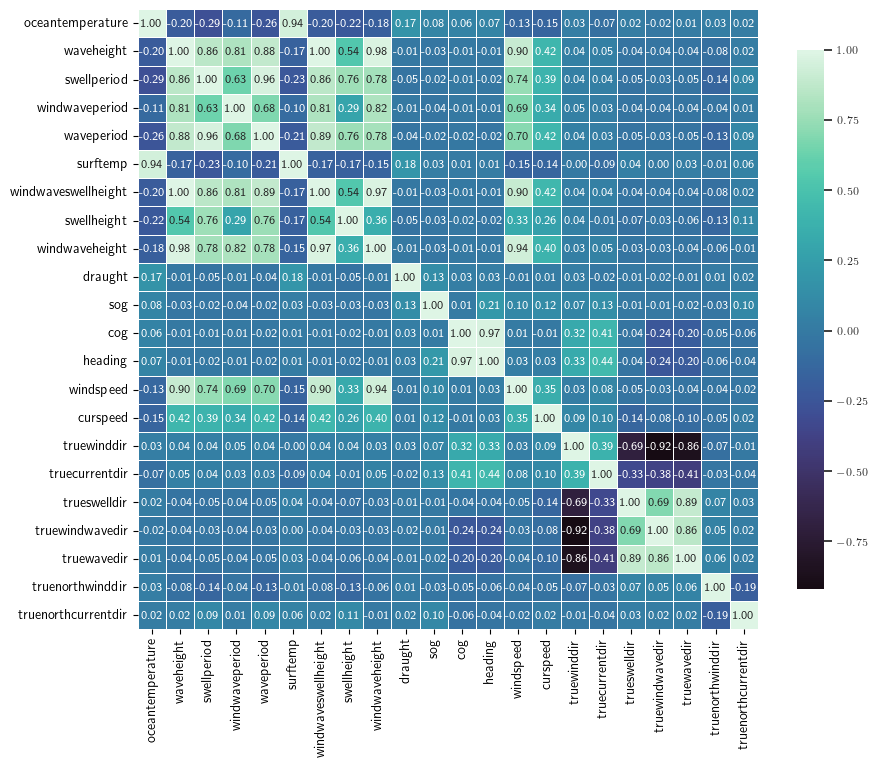
\includegraphics[width=.9\linewidth,height=.9\textheight,keepaspectratio]{02_figures/heatmap_corr_ovr.png}
    \caption{Correlation Heat Map}
    \label{fig:heatmap_ovr}
\end{figure}

From \Cref{fig:heatmap_ovr}, high correlation is observed between wave period, swell period and wind wave period. As discussed in \Cref{sec:weather_definition}, the sea state can be described through the significant height $H_{1/3}$ and spectral peak $T_p$ with help of Torsethaugen peak \bcitep{K.Torsethaugen.2004}. Hence, the features swell period and wind wave period are discarded as it only distinguish whether the sea is dominated by swell or by wind. The feature wave period will still be retained. As a result, the features ``true wind wave direction'' and ``true swell direction'' will be excluded from consideration since the features that account for their magnitude have been discarded.\\

Statistically, the heading and COG are highly correlated, but both features are retained as it explain two different parameters of the ship. Course Over Ground reflects the ship course heading while heading represented the actual heading of the ship at a particular point of time. Same principle also apply between air temperature above ocean and sea surface temperature. Air temperature above oceans represents the temperature of wind while sea surface temperature represents current temperature of current. From feature selection, 5 features from AIS data are discarded while 11 features are removed from the weather data. To predict the ship speed, The SOG will be selected as the label to train the model. The remaining attributes will be selected as training features. This is summarised in \Cref{tbl:struct_train_final}.\\

\begin{table}
    \footnotesize
    \centering
    % \resizebox {\textwidth}{!}
    {\begin{tabular}{ p{8cm}c }
    \hline
    \multicolumn{2}{l}{\textbf{Training Label}}\\
    \hline
    SOG [Knots] & {\tt sog} \\
    \hline
    \multicolumn{2}{l}{\textbf{Training Features}}\\
    \hline
    COG [°] & {\tt cog}  \\
    Heading [°] & {\tt heading}  \\
    Draught [m] & {\tt draught} \\
    Wind Speed [m/s] & {\tt windspeed} \\
    Air Temperature Above Oceans [K] & {\tt oceantemperature} \\
    % Maximum Wave Height [m] & {\tt waveheight} \\
    Wave Period [s] & {\tt waveperiod}\\
    Sea Surface Temperature [K] & {\tt surftemp}\\
    Combined Wind Wave Swell Height [m] &  {\tt windwaveswellheight} \\
    Current Speed [m/s] & {\tt curspeed} \\
    True Wind Direction [°] & {\tt truewinddir}  \\
    True Current Direction [°] & {\tt truecurrentdir} \\
    True Wave Direction [°] & {\tt truewavedir} \\
    \hline
    \end{tabular}}
\caption{Structure of training dataset}\label{tbl:struct_train_final}
\end{table}

\begin{table}
    \footnotesize
    \centering
    % \resizebox {\textwidth}{!}
    {\begin{tabular}{ p{0.23\linewidth} c c c c c c c c }
    \hline
    Features & Count & Mean & Std. & Min & 25\% & 50\% & 75\% & Max \\
    \hline
    \textbf{{\tt sog}} & 2871 & 16.91 & 3.18 & 5.03 & 16.56 & 17.94 & 18.72 & 21.07\\
    \hline
    {\tt cog} & 2871 & 196.47 & 85.93&	69.77 & 102.58& 188.01& 282.26& 355.07\\ 
    {\tt heading} & 2871 & 187.88&	88.47&	67.90&	100.86&	124.65&	279.19&	355.07\\
    {\tt draught} & 2871 &5.22& 0.18& 4.74& 5.11& 5.28& 5.38&5.67\\
    {\tt windspeed} & 2871 & 6.42 & 2.97 & 0.25 & 4.13 & 6.15 &	8.36 & 16.01\\
    {\tt oceantemperature}\tablefootnote{Air temperature above oceans}& 2871 & 282.71 & 6.49 & 264.08& 277.13& 282.64& 288.82& 296.83 \\
    {\tt waveperiod} & 2871& 3.66& 0.82& 1.86& 3.07& 3.57& 4.14& 7.05\\
    {\tt surftemp}\tablefootnote{Sea Surface Temperature}&2871 &283.40& 5.73& 273.05& 278.13& 282.83& 288.86 &294.75\\
    {\tt windwaveswellheight}\tablefootnote{Significant wave height}  &  2871 & 0.75 & 0.51 & 0.07 &0.38 &	0.64 &	0.95 &  3.70  \\
    {\tt curspeed} & 2871 &0.10& 0.07& 0.00 & 0.05& 0.08 & 0.13 & 0.53\\
    {\tt truewinddir} & 2871 & 87.14 & 55.96 &	0.00 & 34.19 &	84.79 & 140.58 & 179.77	\\
    {\tt truecurrentdir} & 2871 & 89.15 & 57.53 & 0.25 & 31.01 & 86.78 & 143.32 & 179.99 \\
    {\tt truewavedir} & 2871 & 91.74 & 55.53& 0.13& 39.12 & 92.28 & 143.33 & 179.92 \\
    \hline
    \end{tabular}}
\caption{Descriptive statistics of preprocessed dataset}\label{tbl:dataset_descriptive_pretraining}
\end{table}

\begin{figure}
    \centering
    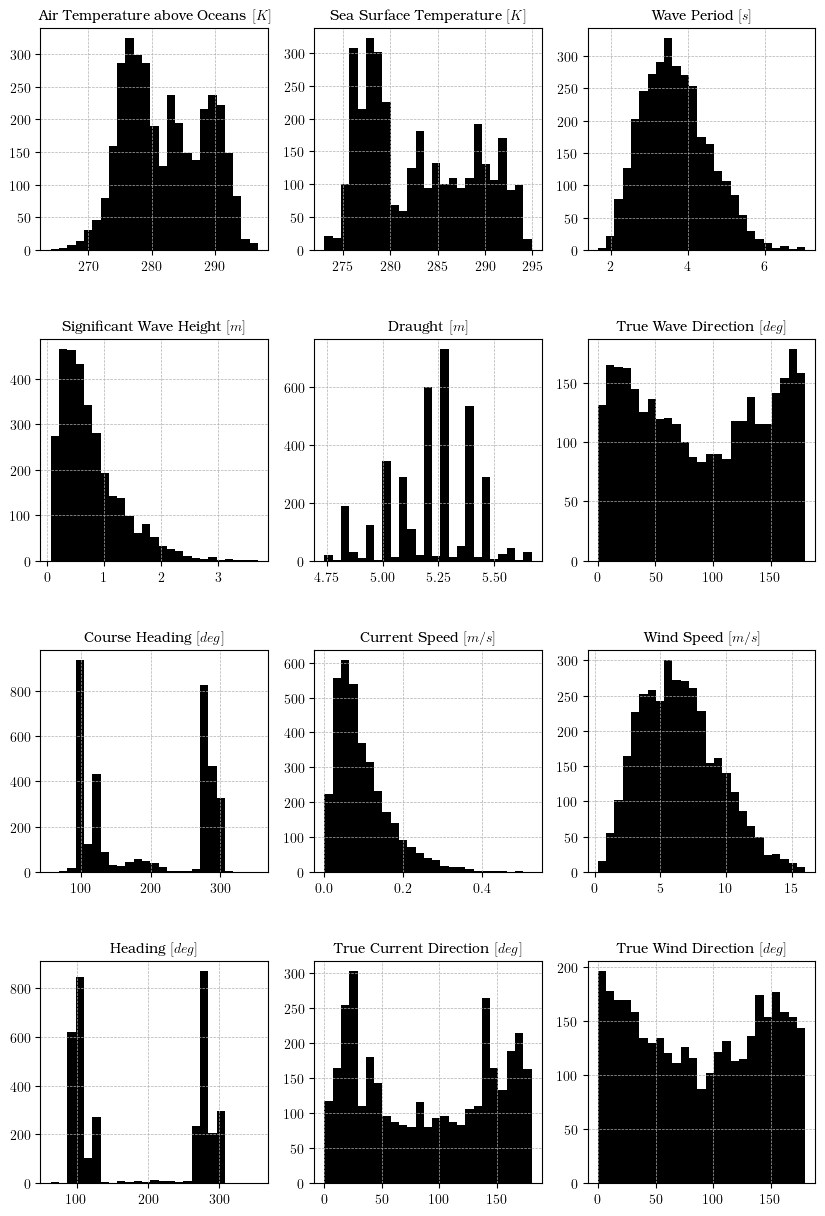
\includegraphics[width=.9\linewidth]{02_figures/hist_init_preprocessing.png}
    \caption{Histogram of training features}
    \label{fig:hist_training_ftr_label}
\end{figure}

\section{Black Box Modelling}\label{sec:BBM_modelling}

In this section, the modelling of ship speed through SOG using selected features will be performed using tree-based regressor model. The tree-based regressor model considered are decision tree regressor (DTR), random forest regressor (RFR) and extra-tree regressor (ETR). The tree-based models are compared against multiple linear regressor (MLR) for benchmarking. For training, the dataset is split into training and test dataset in ratio of 75:25. This corresponds to 2871 data points for training and 957 data points for testing. The training dataset will be subjected to 10-fold splitting, this k-fold splitting is performed as the model will be evaluated using k-fold cross validation. The hyperparameter of the tree-based regressor will be iteratively tuned until no further improvements of the model can be made.\\


\subsection{Performance Metrics for Validation}\label{sec:perf_metrics}

To gain sensible estimate of model performance and how precise a model is, the model will be cross validated by means of k-folding. K-fold cross validation split the training set into k subsets which is called \emph{folds}, then the model will be trained k times using k-1 subsets and remaining one for validation, this process is illustrated in \Cref{fig:kfold}. For each iteration, each model is evaluated using different performance metrics such as \textbf{Coefficient of Determination ($R^2$), Explained Variance (EV), Mean Absolute Error (MAE),Root Mean Square (RMSE), Median Absolute Deviation (MAD) and Mean Absolute Percentage Error (MAPE)}. The results from each iteration is then averaged, where the information on model precision can be gained from the standard deviation. Performing k-fold cross validation checks model robustness against different datasets. The properties of each performance metric will be discussed in the following sections.

\begin{figure}
    \centering
    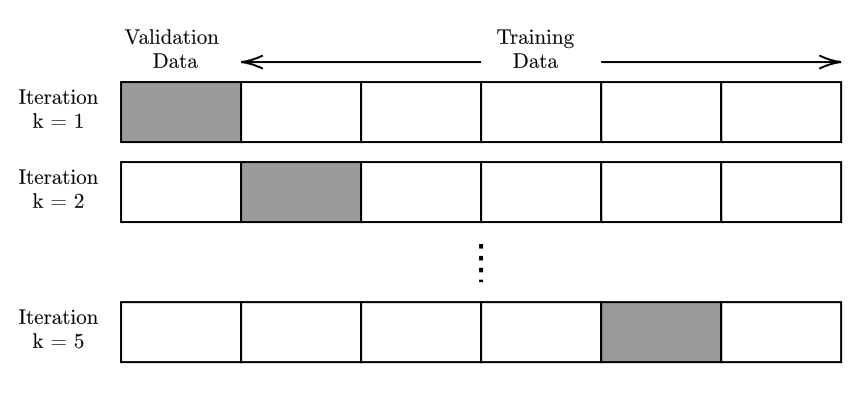
\includegraphics[width=.85\textwidth]{02_figures/kfold.png}
    \caption{Visual illustration of k-folding, Grey shaded box represents the validation data while white box represents the training data}
    \label{fig:kfold}
\end{figure}

\subsubsection*{Coefficient of Determination ({$R^2$})}\label{sec:rsquared}

The coefficient of determination $R^2$ gives a measure on prediction quality, $R^2$ quantifies the ability of the regression model to approximate the actual values. $R^2 $ is defined by \Cref{eqn:rsquared}, where $y$ represents true target output, $\hat{y}$ represents the predictor output and $\overline{y}$ represents the mean. $R^2$ score range between 0 and 1, higher values i.e. $R^2 \rightarrow 1$ indicate better model fit and score of 1 indicate perfect prediction.\\

\begin{equation}\label{eqn:rsquared}
    R^2(y,\hat{y}) = 1 - \frac{\sum_{i = 1}^{n} (y_{\text{i}} - \hat{y}_{\text{i}} )^2 }{\sum_{i = 1}^{n} (y_{\text{i}} - \overline{y}_{\text{i}})^2} \quad \textbf{where} \quad \overline{y} = \frac{1}{n}\sum_{1}^{n} y_\text{i}
\end{equation}

\subsubsection*{Explained Variance (EV)}\label{sec:expVar}

Explained variance indicate how well a model can capture variance from a dataset. It is defined by \Cref{eqn:expVar}, where $\sigma_x$ represents standard deviation of parameter $x$. EV score range between 0 and 1, where the best score of $EV = 1$ can be obtained if $\sigma^2_{(y-\hat{y})} \rightarrow 0$.\\  

\begin{equation}\label{eqn:expVar}
    EV(y,\hat{y}) = 1 - \frac{\sigma^2_{(y-\hat{y})}}{\sigma^2_{y}}
\end{equation}

\subsubsection*{Mean Absolute Error (MAE)}\label{sec:MAE}

MAE indicated the expected value of absolute ($L^1$ norm) error, and it can be calculated by:

\begin{equation}\label{eqn:MAE}
    MAE(y,\hat{y}) = \frac{1}{n}\sum_{i=1}^{n} |y_{\text{i}} - \hat{y}_{\text{i}}| 
\end{equation}

\subsubsection*{Root Mean Square Error (RMSE)}\label{sec:RMSE}

The RMSE describe the expected value of quadratic error. RMSE place large penalty on large deviation between true and estimated values and for this reason, it can be used to as a metric to indicate model performance against outliers. Ideal score is observed when $\text{RMSE} \rightarrow 0$. RMSE can be considered as absolute measure of model fitness. Omitting the root term, RMSE becomes MSE, which is the loss function of \Cref{eqn:costfun} that is used to determine the most optimal split in a regression decision tree.\\

\begin{equation}\label{eqn:RMSE}
    RMSE(y,\hat{y}) = \sqrt{\frac{1}{n}\sum_{i=1}^{n} (y_{\text{i}} - \hat{y}_{\text{i}})^2} 
\end{equation}

\subsubsection*{Median Absolute Deviation (MAD)}\label{sec:MAD} 

MAD is a performance metrics that considers the median of the absolute errors. It is robust to outlier as it only consider median performance

\begin{equation}\label{eqn:MAD}
    MAD(y,\hat{y}) =  \text{median} (|y_{\text{1}} - \hat{y}_{\text{1}}|,\dots,|y_{\text{i}} - \hat{y}_{\text{i}}|)
\end{equation}

\subsubsection*{Mean Absolute Percentage Error (MAPE)}

Is an alternative to MAE, which provide easier interpretation, the result of MAPE can be interpreted according to \Cref{eqn:MAPE} \bcitep{MontanoMoreno.2013}. The usage of MAPE in model evaluation is to get initial estimate, as MAPE comes with some drawback such as instability when $y_i = 0$ and it may lead to biased forecast \bcitep{Gkerekos.2019}. As such, the evaluation of the model performance will be mainly based on MAE and RMSE.    

\begin{equation}\label{eqn:MAPE}
    MAPE(y,\hat{y}) = \frac{1}{n}\sum_{i=1}^{n} \biggl|\frac{y_{\text{i}} - \hat{y}_{\text{i}}}{y_i}\biggr| \cdot 100\%  \quad \textbf{with} \quad \begin{array}{l c}
        \text{MAPE} & \text{Interpretation}\\
        \hline\\
        < 10 & \text{Highly accurate forecasting} \\
        10-20 & \text{Good Forecasting} \\
        20-50 & \text{Reasonable forecasting}\\
        > 50 & \text{Inaccurate forecasting} \\
    \end{array}
\end{equation}

\subsection{Model Hyperparameter Optimisation}\label{sec:hpo}

The subject of parameter tuning was briefly discussed in \Cref{sec:dt_theo}. In \Cref{sec:dt_theo} parameter tuning was applied to decision tree regressor to avoid overfitting by changing the minimum amount of samples a leaf node has. This example implies that altering model hyperparameter will affect the model performance. However, the optimisation of the hyperparameter cannot be performed \emph{a priori} and as such iterative process will be performed until best hyperparameter value is found.\\ 

% \begin{table}[ht]
%     \scriptsize
%     \centering
%     % \resizebox {\textwidth}{!}
%     {\begin{tabular}{ p{0.33\textwidth}p{3cm}p{3cm}p{3cm}  }
%     \hline
%     \multicolumn{1}{c}{\textbf{Model}} & \multicolumn{1}{c}{\textbf{Decision Tree}}  & \multicolumn{1}{c} {\textbf{Random Forest}} & \multicolumn{1}{c}{\textbf{Extra-Trees}}\\
%     \hline
%     Number of trees & \multicolumn{1}{c}{1} & \multicolumn{1}{c}{Many} & \multicolumn{1}{c}{Many}\\
%     Features considered for split at each node &   \multicolumn{1}{c}{All features}  & \multicolumn{1}{c}{Random subset of features} & \multicolumn{1}{c}{Random subset of features} \\
%     Bootstrapping & \multicolumn{1}{c}{Not applied} & \multicolumn{1}{c}{Yes} & \multicolumn{1}{c}{No}\\
%     Split Rule  & \multicolumn{1}{c}{Best split} & \multicolumn{1}{c}{Best split}& \multicolumn{1}{c}{Random split}\\
%     \end{tabular}}
% \caption{Comparison of tree based model from \Cref{sec:tree_intro}}\label{tbl:table_trees}
% \end{table}

\scikit/ offers {\tt GridSearchCV} and {\tt RandomizedSearchCV} to help search for the most optimal hyperparameter. Both solutions operate with similar principle: The selected hyperparameters to be tuned with its value range is evaluated using cross validation to evaluate the best possible combination between the selected hyperparameters. The difference between {\tt GridSearchCV} and {\tt RandomizedSearchCV} lies in how it searches for the best value for the selected hyperparameters: {\tt GridSearchCV} involves construction of grids containing all possible combinations of hyperparameter value in specified range.{\tt RandomizedSearchCV} randomly samples hyperparameter values.\\ 

The exhaustive nature of {\tt GridSearchCV} means that it is computationally costly to perform, especially when there are multiple hyperparameters to be considered and value search space is large. {\tt RandomizedSearchCV} gives more control to computing budget by setting the number of iteration and usually produces more accurate results than {\tt GridSearchCV} approach. \bcitep{Geron.2019,J.Bergstra.2012}. \\

For this reason, the {\tt RandomizedSearchCV} will be employed to search for best possible hyperparameter. However, the limitation of \emph{a priori} knowledge of hyperparameter value still exists. In spite of {\tt RandomizedSearchCV} ability to control the computational budget, it is still takes considerable time to obtain the best hyperparameter value. The computational budget may be spent on searches in unpromising search space. With that, initial exploration on the effect of each hyperparameter on model performance will be performed to give better overview on which search space that should be considered during hyperparameter optimisation. In the next subsections, the effect of tunable hyperparameter of tree-based model from \scikit/ will be explored to give baseline numbers for the search space. RMSE is used as performance metrics as the hyperparameter parameter optimisation done in this thesis aims to reduce the error during prediction. \\ 

\subsubsection*{Number of features}\label{sec:max_features}

Defined with default value as {\tt max\_features=None} in \scikit/. This hyperparameter controls the number of features to be considered when looking for the best split, the default {\tt None} option means it will consider all features. This parameter tuning is available for Decision Tree Regressor, Random Forest Regressor and Extra-Tree Regressor. Initial exploration indicated Random Forest Regressor and Extra Tree Regressor benefit from considering more features, Decision Tree Regressor requires further fine-tuning to optimise the model as the default {\tt None} means it will consider all features when searching for best split.\\ 

\begin{figure}[h]
    \centering
        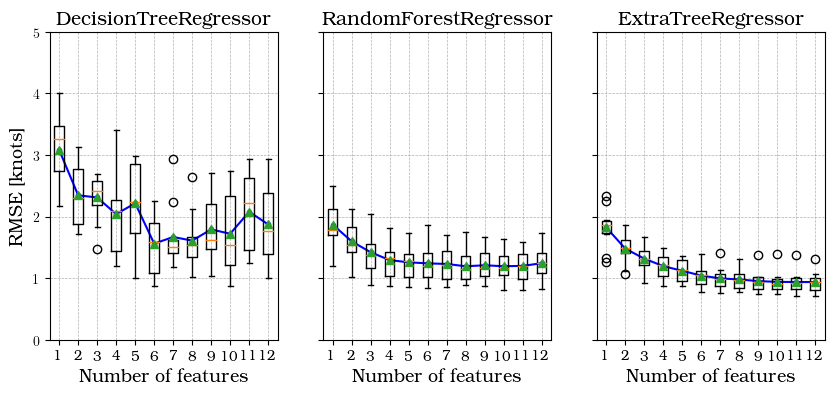
\includegraphics[width=.9\textwidth]{02_figures/hpo_n_features.png}
        \caption{Hyperparameter tuning of {\tt max\_features}}
        \label{fig:hpo_n_features}
\end{figure}

\subsubsection*{Minimum samples to split a node}\label{sec:min_samples_split}

Defined with default value as {\tt min\_samples\_split=2} in \scikit/. This hyperparameter controls the minimum number of samples i.e. data points required to split a node. The default value of {\tt 2} is the least number of sample required to split a node i.e. 1 sample is split to the left and right branch respectively. The plot at \Cref{fig:hpo_min_samples_leaf} indicates that neither RF nor ET benefits from this tuning parameter, as they constructed based on ensemble of uncorrelated tree and this parameter will affect the performance of individual tree in the forest. Whereas, the break even point for the tuning value is found at {\tt min\_samples\_split=20}.  
\begin{figure}[h]
    \centering
        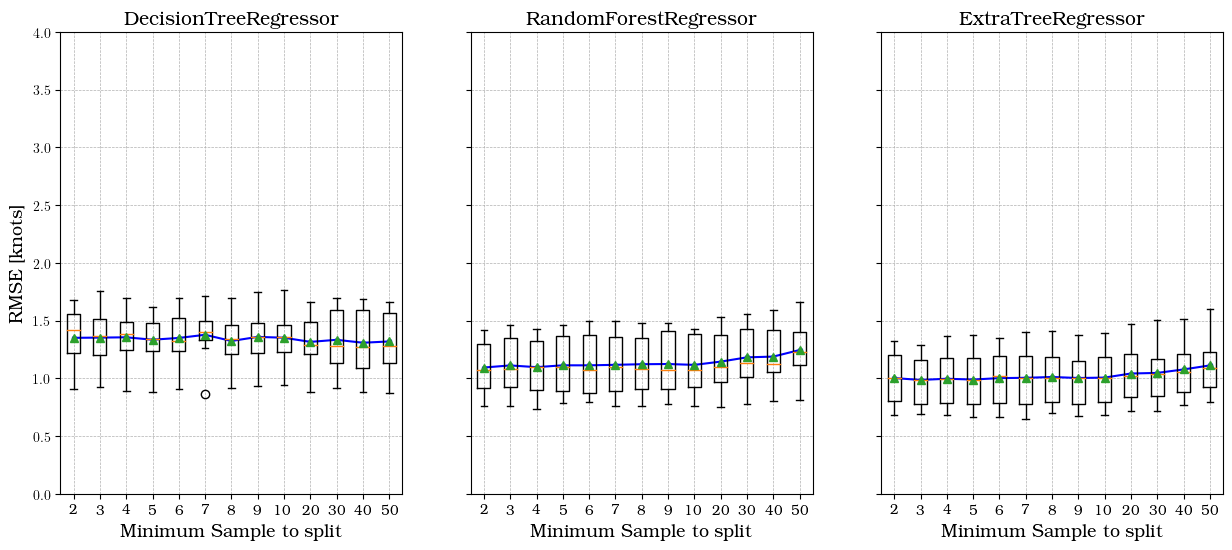
\includegraphics[width=.9\textwidth]{02_figures/hpo_min_samples_split.png}
        \caption{Hyperparameter tuning of {\tt min\_samples\_split}}
        \label{fig:hpo_min_samples_split}
\end{figure}


\subsubsection*{Number of sample in a leaf node}\label{sec:min_samples_leaf}

Defined with default value as {\tt min\_samples\_leaf=1} in \scikit/. This parameter controls number of samples required to be at leaf node, where split point will be considered if the leaf contains at least {\tt min\_samples\_leaf=n} training samples in each left and right branch. As shown in \Cref{fig:geron6_6}, tuning this hyperparameter to higher values helps to smoothen the model and avoid overfitting. However, this may lead to underfitting as the model is unable to capture the trend within the data. This is supported by the findings shown in \Cref{fig:hpo_min_samples_leaf}, the DTR benefits from regularisation at certain breakeven point, in this case, it is found to be at {\tt min\_samples\_leaf=4}. But after this breakeven point, the model's performance degrades. It is also observed that RFR and ETR does not benefit from any form of regularisation.  

\begin{figure}[h]
    \centering
        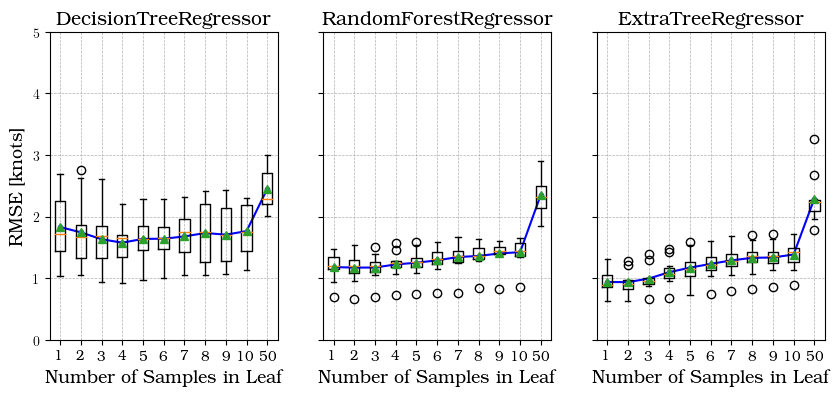
\includegraphics[width=.9\textwidth]{02_figures/hpo_min_samples_leaf.png}
        \caption{Hyperparameter tuning of {\tt min\_samples\_leaf}}
        \label{fig:hpo_min_samples_leaf}
\end{figure}

\subsubsection*{Depth of Tree}\label{sec:max_depth}

Defined with default value as {\tt max\_depth=None} in \scikit/. This hyperparameter controls the growth of the tree. Leaving it at {\tt max\_depth=None} means the tree will grow until all leaves are pure i.e. until minimum MSE is obtained or when the number of samples is less than the minimum number of samples required to split an internal node. Similar to {\tt min\_samples\_leaf}, DTR shows improvement until a certain breakeven point. RFR performance seems to stabilise at certain depth while ETR benefits from allowing full growth of the tree. The results are summarised in \Cref{fig:hpo_max_depth}  

\begin{figure}[h]
    \centering
        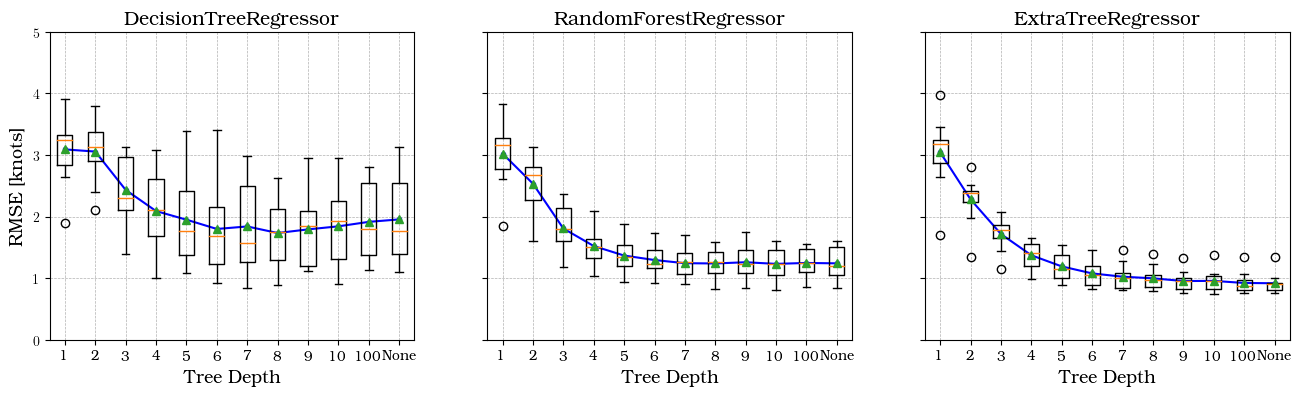
\includegraphics[width=.9\textwidth]{02_figures/hpo_max_depth.png}
        \caption{Hyperparameter tuning of {\tt max\_depth}}
        \label{fig:hpo_max_depth}
\end{figure}

\subsubsection*{Number of Trees}\label{sec:n_estimators}

Defined with default value as {\tt n\_estimators=100}. This hyperparameter controls the amount of trees i.e. predictors in a forest. Tuning of number of trees will have an effect on the training time and it is only available to RFR and ETR. The default value seems to yield satisfactory result, as the performance for both RFR and ETR stabilise after in this case stabilise after 100 trees, as seen in \Cref{fig:hpo_n_features}. 

\begin{figure}[h]
    \centering
        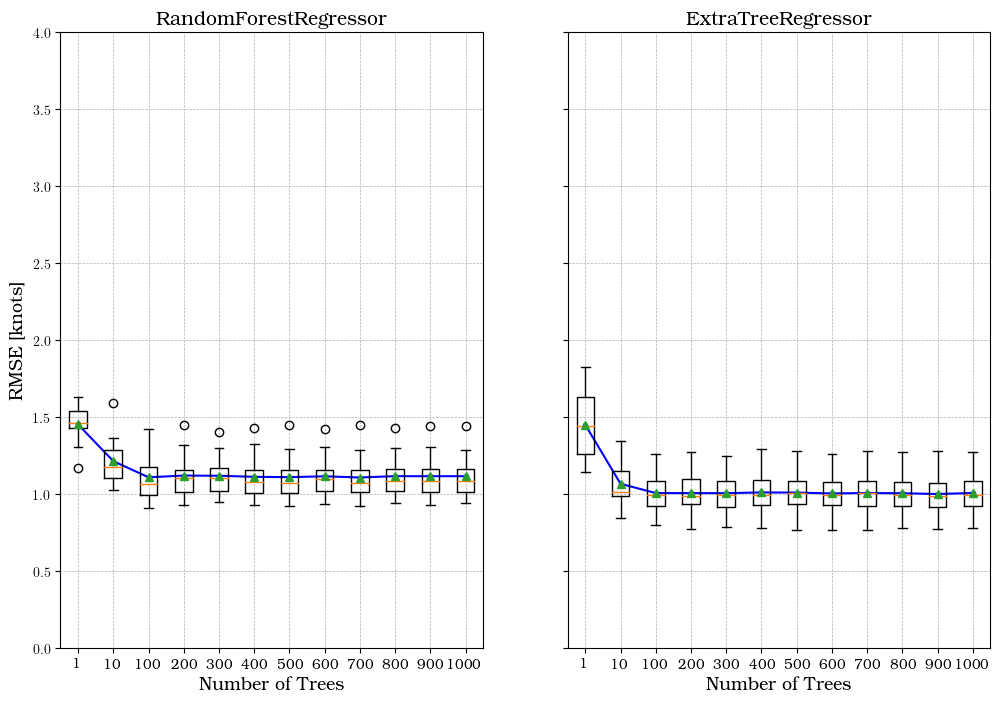
\includegraphics[width=.65\textwidth]{02_figures/hpo_n_estimators.png}
        \caption{Hyperparameter tuning of {\tt n\_estimators}}
        \label{fig:n_estimators}
\end{figure}


% \begin{figure}
%     \centering
%         \includegraphics[width=.85\textwidth]{02_figures/JuneFilter.png}
%         \caption{Journey of the ship in June}
%         \label{fig:JuneJourney}
% \end{figure}

\section{White Box Modelling}\label{sec:WBM_modelling}

In this section, the predicted SOG from the BBM will be fed into the WBM to predict the fuel consumption (FOC). Using Holtrop-Mennen approximation method, the resistance encountered by the ship will be estimated to find the total resistance which will be used to calculate the power required to propel the ship. However, during resistance calculation, some form coefficients and ship parameters are not readily available and may need to be assumed based on other literature studies, this assumption will be indicated throughout this section. The resulting brake power $P_B$ is plotted against the STW $v_S$ to obtain a power speed curve model which can be used to predict FOC. 

\subsection{Calculation of Total Resistance}\label{sec:Rtot_calc_method}

The formula used to calculate total resistance $R_{TOTAL}$ in this section are presented in \Cref{sec:holtrop_mennen_calc} with principle dimension of the ship which was given in \Cref{tbl:Hammershus_Data}. Some assumptions are made for the sea state and the values of some form coefficients are calculated based on empirical formulas presented in \Cref{sec:Ship_design_param}. In this case study, Holtrop-Mennen method can be used as it fulfills the condition set in \Cref{eqn:holtrop_cond}:
\begin{equation}
    \label{eqn:holtrop_cond_fulfill}
    % \begin{multlined}
    \begin{gathered}
        Fr = 0.2417  \leqslant 0.45 \\
        0.55 \leqslant C_P = 0.6707 \leqslant 0.85 \\
        3.9 \leqslant \frac{L}{B} = 5.91 \leqslant 9.5
    \end{gathered}
    % \end{multlined}
\end{equation}

The calculations of resistance are dynamics as the Froude number $Fr$ is based on $v_S$, the design Froude number $Fr_{DESIGN}$ is used to check use cases for some equations.

\subsubsection*{Calculation of frictional resistance $R_F$}

For the calculation of surface area of bare hull $S$, it is assumed that the aft has a U-shaped section. Then the appropriate $C_{stern}$ can be calculated to obtain the constant $c_{14}$ \Cref{eqn:c_14}. For the calculation of length of run $L_R$, approximation for $\ell_{CB}$ are made based on \Cref{eqn:lcb}. The constants $c_{14}$ and $L_R$ are used to calculate the form factor $1+k_1$ which will be used to calculate $R_F$.

\subsubsection*{Calculation of appendage resistance $R_{APP}$}

From known ship information and ship schematics shown in \Cref{fig:Hammershus_Pict}, it can be deducted that the ship consists of the following appendages:

\begin{itemize}
    \setlength\itemsep{0em}
    \item Two high-lift flap rudders
    \item Single centre skeg
    \item Twin shafts supported by two brackets
\end{itemize}

The assumptions for the appendage area are made by scaling the schematics to known measurements (e.g. the $L_{WL}$). From here, the appropriate $k_{2_i}$ constants for individual appendages will be selected to obtain the $(1+k_{2_i})_{eq}$ from \Cref{eqn:k2eq}.

\begin{table}[ht]
    \footnotesize
    \centering
    % \resizebox {\textwidth}{!}
    {\begin{tabular}{ p{0.2\linewidth} c c}
    \hline
    Appendage type & Value & $(1+k_{2_i})$ \\
    \hline
    \multicolumn{2}{l}{\textbf{Two high-lift flap rudders}} & 3\\
    \hline
    $h_{\text{RUDDER}}$ & 4.06 $m$\\
    $B_{\text{RUDDER}}$ & 1.99 $m$\\
    $S_{\text{RUDDER}}$ & 16.16 $m^2$\\
    \hline
    \multicolumn{2}{l}{\textbf{Single centre skeg}} & 1.5\\
    \hline
    $h_{\text{SKEG}}$ & 4.41 $m$\\
    $B_{\text{SKEG}}$ & 26.23 $m$\\
    $S_{\text{SKEG}}$ & 115.67 $m^2$\\
    \hline
    \multicolumn{2}{l}{\textbf{Twin shafts supported by two brackets}} & 3\\
    \hline
    $D_{\text{SHAFT}}$ & 0.55 $m$\\
    $L_{\text{SHAFT}}$ & 13.54 $m$\\
    $S_{\text{SHAFT}}$ & 46.79 $m^2$\\
    \hline
    \multicolumn{1}{l}{\textbf{$S_{APP_{tot}}$}} & \textbf{178.62} $m^2$ \\
    \multicolumn{2}{l}{\textbf{$(1+k_{2_i})_{eq}$}} & \textbf{2.03} \\
    \end{tabular}}
\caption{Assumed appendage values}\label{tbl:assume_appendage_dimension}
\end{table}

Additionally, there are two bow thrusters installed with approximated diameter of $d_{TH}= 2.15 m$, from here, the constant $C_{D_TH}$ can be approximated using \Cref{eqn:R_th}. Hence, the appendage resistance $R_{APP}$ can be calculated using \Cref{eqn:R_app}.

\subsubsection*{Calculation of wave resistance $R_{W}$}

The calculation of wave resistance is based on the case for $Fr \leq 0.4$ using equation \Cref{eqn:R_w_low}. The estimation is done by adding the constants presented between \Cref{eqn:c_7} and \Cref{eqn:m4}. There are some use cases for some equations, which is summarised in \Cref{tbl:R_w_use_case}.

\begin{table}[ht]
    \footnotesize
    \centering
    % \resizebox {\textwidth}{!}
    {\begin{tabular}{ p{0.2\linewidth} c c }
    \hline
    Constant & Use Case & Equation \\
    \hline
    $c_7$ &  $0.11 < \frac{B}{L_{WL}} \leq 0.25$ & \Cref{eqn:c_7} \\
    $c_{15}$ & $\frac{L_{WL}^2}{V} \leq 512$ & \Cref{eqn:c15} \\
    $c_{16}$ & $C_P \leq 0.8$ & \Cref{eqn:c16} \\
    $\lambda$ & $L_{WL} \leq 12$ & \Cref{eqn:lambda} \\
    \hline
    \end{tabular}}
\caption{Use case of constants for $R_W$}\label{tbl:R_w_use_case}
\end{table}

\subsubsection*{Calculation of bulbous bow resistance $R_B$}
The area $A_{BT}$ used to calculate is approximated based on \bcitet{Kracht.78} with:

\begin{equation}
    \label{eqn:A_BT}
    A_{BT} = 0.085 A_M
\end{equation}

For the height $h_B$, the upper limit of $h_B = 0.6T_{DESIGN}$ is selected, and it is assumed that $T_F = T_{DESIGN}$.

\subsubsection*{Calculation of (immersed) transom resistance $R_{TR}$}

Since the immersed transom area is unknown, \bcitet{Rakke2016} approximated the immersed transom area based on correlation of ship dimension from literature review of \bcitet{Holtrop.1982}:

\begin{equation}
    \label{eqn:A_M}
    A_{TR} = 0.051 A_M
\end{equation}

This approximation must be used with caution as it is only based on case study of \bcitet{Holtrop.1982}. However, to author's best knowledge, there are no other literature that provide empirical estimation of $A_{TR}$. Therefore, this estimation will be selected in this case study. The selection for the value of constant $c_6$ is dependent on the value of $Fr_T$, which is a function of $v_S$. From there, the transom resistance can be calculated using \Cref{eqn:R_transom}

\subsubsection*{Calculation of correlation allowance resistance $R_A$}

The selection of constant $c_4$ in equation \Cref{eqn:c4} is based on the $T_F$, then the correlation resistance $R_A$ can be calculated using \Cref{eqn:R_a}.

\subsubsection*{Calculation of added resistance due to wind $R_{AA}$}

Two assumptions are made during the calculation of $R_{AA}$, since the information of lateral area $A_L$ and $A_F$ are not readily available, these values are assumed based on the dimension of similar ferry in the case study of \bcitet{Blendermann.1994}. It is assumed that the ferry has an $A_L$ of \textbf{2125.80} $m^2$ and $A_F$ of \textbf{325.30} $m^2$. From \Cref{tbl:BlendermannCoeff}, the case for ferry ship is taken to get the necessary constants for the calculation of $R_{AA}$. 

\subsubsection*{Calculation of added resistance due to wave $R_{AW}$ }

This part of the equation is relatively straightforward, $L_{BWL}$ will be approximated to about \textbf{43.75} m. The calculation of $R_{AWL}$ will be based on the data of significant wave height $H_{1/3}$ from the dataset.

\subsection{Calculation of total efficiency $\eta_{TOT}$}\label{sec:eta_tot_method}

\subsubsection*{Calculation of open water efficiency $\eta_O$}

This value is approximated based on the line of Wageningen series in \Cref{fig:breslin_open water efficiencies} \bcitep{Breslin.1994}. The case will be for ``Passenger ships and high speed naval vessels''. Since the value of $C_Th$ is not available, the value of $\eta_O$ is approximated as \textbf{0.7}.

\subsubsection*{Calculation of hull efficiency $\eta_H$}

For the calculation of $\eta_H$, the value of the propeller diameter $D$ is approximated as \textbf{4 m}, which is based on the schematics of the ship shown in \Cref{fig:Hammershus_Pict}.

\subsubsection*{Calculation of relative rotative efficiency $\eta_R$}

The missing value required to compute \Cref{eqn: eta_rot_holtrop} is the pitch-diameter propeller ratio. This value will be estimated as $P/D =$ \textbf{1.135}, which is obtained from the work of \bcitet{Bertram.2000}.

\begin{figure}[h]
    \centering
        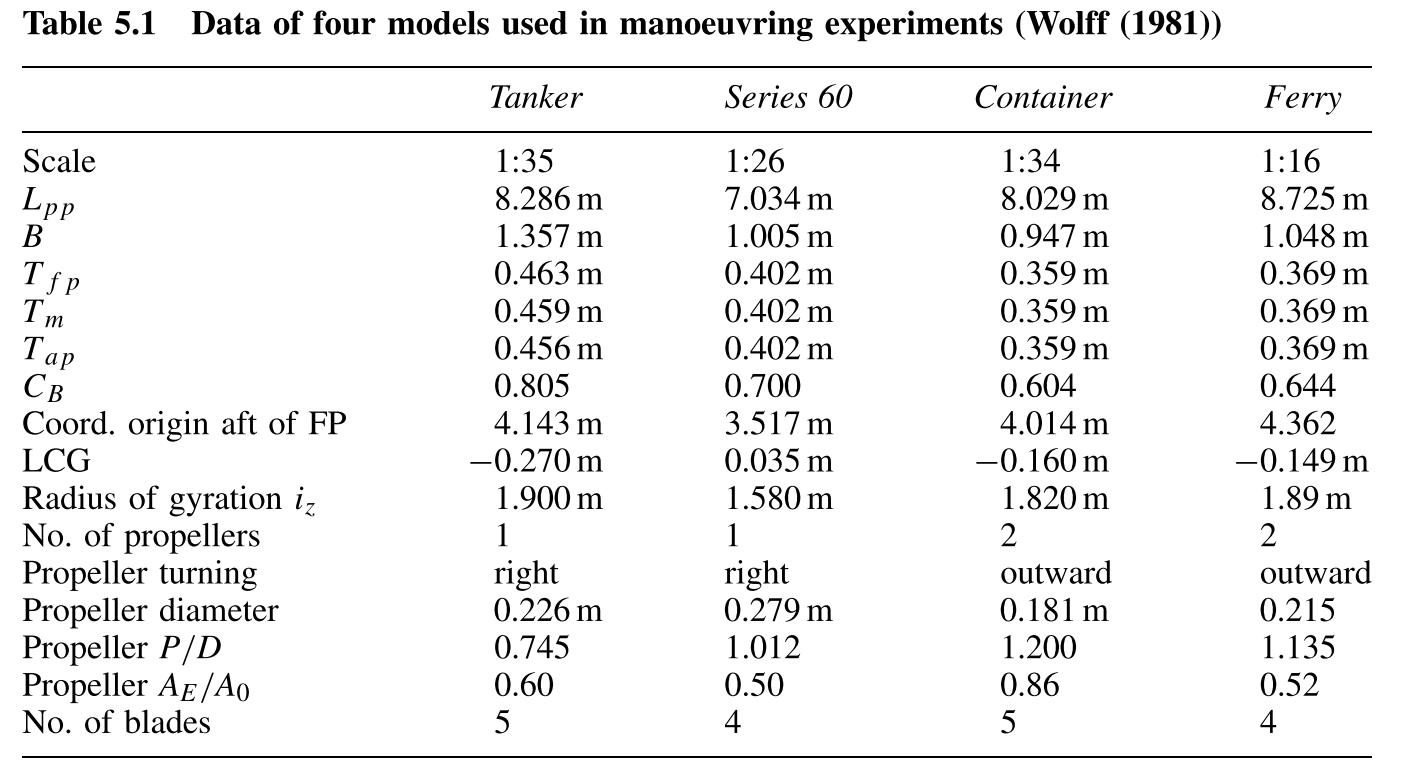
\includegraphics[width=.95\textwidth]{02_figures/betram_wolff_ratiomodel .jpg}
        \caption{Estimated value of propeller dimensions}
        \label{fig:betram_wolff_propellerdimensions}
\end{figure}

\subsubsection*{Calculation of shaft efficiency $\eta_S$}

The value of shaft efficiency is estimated as $\eta_S =$ \textbf{0.99} based on \bcitet{Diesel.2011} and \bcitet{Holtrop.1982}.

\subsection{Calculation of FOC}\label{sec:FOC_calc_method}

Once $R_{TOTAL}$ and $\eta_{TOTAL}$ is obtained, then the brake power of the ship $P_B$ can be calculated using \Cref{eqn:P_b}. The resulting $P_B$ will be plotted against $v_S$ to obtain a power-speed curve, then regression line will be constructed to fit the data points. Each of the BBM model will generate different prediction for SOG, the resulting equation of the regression line represents the characteristic of different BBM model. To compare the performance, the regression model from each BBM will be compared against the regression model generated from real data to assess the predictive performance of each model.\\

The FOC can be calculated using \Cref{eqn:FOC}. The information of the SFOC can be obtained from \Cref{tbl:Hammershus_Data}. Without the multiplication with operation time, $\mathcal{T}_{operation}$, The fuel consumption of the fuel in $T/h$ can be obtained by dividing the value by \textbf{$1 \cdot 10^6$}.\\  


\begin{table}
    \footnotesize
    \centering
    % \resizebox {\textwidth}{!}
    {\begin{tabular}{ p{0.1\linewidth} p{0.2\linewidth} p{0.6\linewidth}}
    \hline
    Parameter & Value & Remarks \\
    \hline
    $g$ & 9.805 $kg/ms^2$ \\
    $\rho_{sea}$ & 1025 $kg/m^3$ \\
    $\nu_{sea}$ & 0.00000118 $m^2/s$ \\
    $\rho_{air}$ & 1.25 $kg/m^3$ \\
    1 m/s & 1.9438 knots \\
    \hline
    \multicolumn{3}{l}{\textbf{Required Parameters for Holtrop-Mennen}}\\
    \hline
    $L_{WL}$ & 144.80 m & From \Cref{tbl:Hammershus_Data} \\
    $B$ & 24.50 m & From \Cref{tbl:Hammershus_Data} \\
    $T$ & 5.85 m & Assume $T_A = T_F = T$ for initial phase, otherwise use $T$ from dataset \\
    $Fr_{N}$ & 0.2417 & From \Cref{eqn:Froude_Number} \\
    $C_B$ & 0.6549 & From \Cref{eqn:Cb_Schneekluth}\\
    $C_M$ & 0.9764 & From \Cref{eqn:CM_jensen} \\
    $C_P$ & 0.6707 & From \Cref{eqn:cp_ratio}\\
    $C_{WP}$ & 0.7700 & From \Cref{eqn:cwp_Schneekluth}\\
    $V$ & 13592.1413 $m^3$ & $V = C_B \cdot L_{WL} \cdot T_{MAX}$\\
    $\frac{L_{WL}}{B}$ & 5.9102 \\
    \hline
    \end{tabular}}
\caption{Assumed value for some constants}\label{tbl:assume_sea_constants}
\end{table}


